\chapter[Conformal Group in Two Dimensions]{Conformal Group in \\Two Dimensions}

If the dimension of spacetime is larger than two (\(D>2\)), the conformal group is a finite-dimensional Lie group. While it is larger than the standard Poincar\'e group therefore providing more constraints on the theory, the number of these constraints remains strictly finite. However, in exactly two dimensions, the situation changes drastically and \uline{the conformal symmetry becomes infinite-dimensional}. The two-dimensional case is thus special because the condition for conformal invariance is much more powerful.

This dramatic enhancement makes CFT\(_2\) exactly solvable in many cases. All these results were established in a seminal breakthrough paper by Belavin, Polyakov and Zamolodchikov in 1984 [3] and later reviewed in Lecture notes by Ginsparg [4] and by Cardy [5] and in books by Di Francesco, Mathieu and Sénéchal [6] and by Mussardo [7] and in many other contributions. \TODO{add references.}

To see this, let us work in 2D Euclidean space (if we start from a Minkowski metric, we can always perform a Wick rotation). In a 2D Minkowski spacetime, the natural variables would be the \textit{lightcone coordinates}; in Euclidean space, the analogous operation is to map the 2D Cartesian plane into the complex plane.

\subsubsection{Complex Coordinates}

We take a new basis by changing coordinates from the real Cartesian coordinates \(x^1\) and \(x^2\) to the complex coordinates \(z\) and \(\bar{z}\):
\[
    \begin{dcases}
        z = x^1 + i x^2, \\
        \bar{z} = x^1 - i x^2,
    \end{dcases} \implies \begin{dcases}
        x^1 = \frac{z + \bar{z}}{2}, \\
        x^2 = \frac{z - \bar{z}}{2i}.
    \end{dcases}
\]
While physically one coordinate is the complex conjugate of the other, it is mathematically very convenient to treat \(z\) and \(\bar{z}\) as two formally independent variables characterizing a point in \(\mathbb{C}^2\).

In these new coordinates, the flat Euclidean line element becomes:
\[
    \mathrm{d} s^2 = (\mathrm{d} x^1)^2 + (\mathrm{d} x^2)^2 = \mathrm{d} z \mathrm{d} \bar{z},
\]
where \(\mathrm{d} z \mathrm{d} \bar{z}\) also acts as the area element (\(\mathrm{d}^2 \mathbf{x}\)) up to a constant factor. The corresponding derivatives with respect to the complex coordinates are given by:
\[
    \begin{dcases}
        \partial_z = \frac{1}{2}(\partial_1 - i \partial_2), \\
        \partial_{\bar{z}} = \frac{1}{2}(\partial_1 + i \partial_2),
    \end{dcases} \quad \implies \quad \begin{dcases}
        \partial_z z = 1, \quad \partial_z \bar{z} = 0, \\
        \partial_{\bar{z}} z = 0, \quad \partial_{\bar{z}} \bar{z} = 1.
    \end{dcases}
\]
From the line element \(\mathrm{d}s^2 = g_{\mu\nu}\mathrm{d}x^\mu \mathrm{d}x^\nu\), we can read off the metric tensor in the \((z, \bar{z})\) basis, which takes the off-diagonal form:
\[
    g = \begin{pmatrix}
        0            & \tfrac{1}{2} \\
        \tfrac{1}{2} & 0
    \end{pmatrix}.
\]
Consequently, any field in our theory can be redefined as a function of these two independent variables in the complex plane:
\[
    \varphi(x) \to \varphi(z, \, \bar{z}),
\]
letting us treat the two-dimensional space as a complex manifold. This choice of coordinates is not just a mathematical convenience; it is crucial for revealing the rich structure of conformal transformations in two dimensions, which are intimately connected to the properties of analytic functions.

With these tools at our disposal, we can now analyze the conformal transformations in two dimensions and their profound implications for the structure of the theory.

\section{Conformal Transformations in Two Dimensions}

Let us now consider conformal transformations. A coordinate transformation is conformal if it simply rescales the line element by a strictly positive local factor \(\Omega\):
\[
    (\mathrm{d}s^{\prime})^2 =  \Omega^2(z, \, \bar{z}) \mathrm{d} s^2,
\]
which means \textit{the transformation is preserving the metric up to a local scaling}. This is a much weaker condition than the isometry condition, which requires the metric to be invariant under the transformation. The conformal condition allows for a much larger class of transformations, as it only requires angles to be preserved locally, while lengths can be rescaled by an arbitrary function.

In complex coordinates, we can achieve this by applying independent transformations to \(z\) and \(\bar{z}\). Then the idea is to solve the conformal condition locally introducing the following analytic maps:
\[
    \begin{dcases}
        z \mapsto w = f(z), \\
        \bar{z} \mapsto \bar{w} = \bar{f}(\bar{z}),
    \end{dcases} \quad \implies \quad \begin{dcases}
        \mathrm{d} w = f^{\prime}(z) \mathrm{d} z, \\
        \mathrm{d} \bar{w} = \bar{f^{\prime}}(\bar{z}) \mathrm{d} \bar{z}.
    \end{dcases}
\]
Here, \(f(z)\) is an analytic (holomorphic) function, meaning its derivative \(f'(z)\) exists, and \(\bar{f}(\bar{z})\) is an anti-holomorphic function. The new line element becomes:
\[
    (\mathrm{d} s^{\prime} )^2 = \mathrm{d} w \mathrm{d} \bar{w} = f^{\prime}(z) \bar{f^{\prime}}(\bar{z}) \mathrm{d} z \mathrm{d} \bar{z},
\]
which perfectly matches the conformal condition with the scale factor completely factorized into a holomorphic and an anti-holomorphic part:
\[
    \Omega^2(z, \, \bar{z}) = f^{\prime}(z) \bar{f^{\prime}}(\bar{z}).
\]
This reveals a profound result: \uline{\textit{any} analytic transformation of the complex plane is a conformal transformation}. Geometrically, analytic functions preserve local angles, maintaining the shape of infinitesimally small figures, even though globally they can stretch and severely distort areas.

Since there are infinitely many analytic functions, the conformal group in two dimensions is \textbf{infinite-dimensional}. This implies we have infinitely many symmetries and, consequently, infinitely many constraints on the algebra of local fields. When a theory is subjected to infinitely many constraints, it often becomes exactly solvable, allowing us to compute quantities far beyond standard perturbation theory.

\subsection{Infinitesimal Conformal Transformations}

To rigorously link this to the conformal Killing equation, consider an infinitesimal conformal map:
\[
    \begin{aligned}
        z       & \mapsto z + \epsilon(z),                   \\
        \bar{z} & \mapsto \bar{z} + \bar{\epsilon}(\bar{z}),
    \end{aligned}
\]
where \(\epsilon(z)\) and \(\bar{\epsilon}(\bar{z})\) are infinitesimal holomorphic and anti-holomorphic functions, respectively. We define the displacement vector components as:
\[
    \epsilon(z) = \epsilon_1 + i \epsilon_2, \quad \bar{\epsilon}(\bar{z}) = \epsilon_1 - i \epsilon_2.
\]
By definition, an infinitesimal transformation is conformal if it satisfies the conformal Killing equation. In \(D=2\) dimensions, this equation reads:
\begin{equation}
    \partial_\mu \epsilon_\nu + \partial_\nu \epsilon_\mu = \frac{2}{2} (\partial \cdot \epsilon) \delta_{\mu\nu} = (\partial_1\epsilon_1 + \partial_2\epsilon_2) \delta_{\mu\nu}.
    \label{eq:conformal_killing_equation_2d}
\end{equation}
Evaluating this tensor equation component by component (\((\mu, \nu)=(1,1)\), \((2,2)\) and \((1, 2)\)), we obtain exactly the celebrated \textbf{Cauchy-Riemann equations}:
\begin{equation}
    \begin{dcases}
        \partial_1 \epsilon_1 = \partial_2 \epsilon_2, \\
        \partial_1 \epsilon_2 = -\partial_2 \epsilon_1.
    \end{dcases}
    \label{eq:cauchy_riemann_equations_2d}
\end{equation}
These equations are the necessary and sufficient condition for \(\epsilon(x^1, x^2) = \epsilon_1 + i \epsilon_2\) to be a complex analytic function \(\epsilon(z)\). This confirms that in two dimensions, the set of all conformal transformations coincides precisely with the set of all holomorphic and anti-holomorphic mappings.

Furthermore, if we were to write the Cauchy-Riemann equations in complex coordinates, we would find that they reduce to the simple conditions:
\[
    \begin{aligned}
        \partial_{\bar{z}} \epsilon(z, \bar{z}) & = 0 \quad \implies \epsilon(z, \bar{z}) = \epsilon(z),                   \\
        \partial_z \bar{\epsilon}(z, \bar{z})   & = 0 \quad \implies \bar{\epsilon}(z, \bar{z}) = \bar{\epsilon}(\bar{z}),
    \end{aligned}
\]
which explicitly shows that the holomorphic and anti-holomorphic sectors are completely decoupled, and the conformal transformations can be treated independently in each sector. This factorization is a fundamental structural property of two-dimensional conformal field theory.

Since \(\epsilon(z)\) is analytic, it can be expanded in a Laurent series around any point in its domain of analyticity (for simplicity, we can choose the origin \(z=0\)) as:\footnote{More rigorously, any function holomorphic in an annulus $r < |z| < R$ admits a unique Laurent expansion that converges uniformly on compact subsets of the annulus. The existence of this series is a direct mathematical consequence of holomorphy in that domain, without requiring additional global assumptions about the function's boundedness or divergence.}
\[
    \epsilon(z) = \sum_{n = -\infty}^{\infty} \epsilon_n z^{n + 1}.
\]
This series represents the most general form of such an analytic function and is convergent within its specific annulus of convergence. By isolating the terms of this expansion, we can extract a convenient basis of infinitesimal holomorphic transformations:
\[
    \epsilon_n(z) = - z^{n + 1}, \quad n \in \mathbb{Z},
\]
then the generators of the transformations on scalar fields \(\varphi(x)\) as
\[
    \ell_n = - z^{n + 1} \partial_z, \quad \bar{\ell}_n = - \bar{z}^{n + 1} \partial_{\bar{z}},
\]
where the generators for the other sector were derived by the same reasoning, but in the \(\bar{z}\) direction. The generators \(\ell_n\) and \(\bar{\ell}_n\) form a convenient basis for the infinite-dimensional algebra of conformal transformations in two dimensions.

We now compute the commutator $[\ell_n, \ell_m]$ to determine the structure constants of the algebra. By applying the operators to a test function $f(z)$, we obtain:
\begin{equation}
    [\ell_n, \ell_m] = (n - m) z^{n + m + 1} \partial_z = (n - m) \ell_{n + m}
    \label{eq:witt_algebra}
\end{equation}
This relation defines the \textbf{Witt algebra}, which is the algebra of infinitesimal conformal transformations in two dimensions. The exact same commutation relation holds for the anti-holomorphic generators $\bar{\ell}_n$. Because the indices $n$ and $m$ can take any integer value, this forms an infinite-dimensional Lie algebra, which along with the other sector's algebra, constitutes the full symmetry algebra of two-dimensional conformal field theories:
\begin{equation}
    [\ell_n, \ell_m] = (n - m) \ell_{n + m}, \quad [\bar{\ell}_n, \bar{\ell}_m] = (n - m) \bar{\ell}_{n + m}, \quad [\ell_n, \bar{\ell}_m] = 0.
    \label{eq:2d_cft_witt_algebra}
\end{equation}

The Witt algebra serves as the classical precursor to the Virasoro algebra, which represents the quantum version of the 2D conformal algebra. As an interesting historical note, Miguel Virasoro introduced this algebraic structure in 1970 in the context of early string theory (dual resonance models), as a PhD student in Turin. Furthermore, while the global conformal transformations (the Möbius transformations, which we will introduce shortly) had already been known for over a century in classical mathematics, Virasoro's profound contribution was uncovering the physical relevance of this infinite-dimensional algebra.

\subsection{Global Conformal Transformations}

Not all holomorphic maps are globally well-defined on the Riemann sphere. The globally defined conformal transformations, i.e. those mapping a plane into a plane, are the Möbius transformations:
\begin{equation}
    z \mapsto w = \frac{az + b}{cz + d}, \quad ad - bc = 1,
    \label{eq:mobius_transformations}
\end{equation}
which form a six-parameter family of transformations. These transformations are generated by the three generators \(\ell_{-1}\), \(\ell_0\) and \(\ell_1\) (and their anti-holomorphic counterparts), which correspond to the following specific transformations:
\begin{enumerate}
    \item \(\ell_0 = -z \partial_z\) is the generator of \textbf{dilatations} and \textbf{rotations},
    \item \(\ell_{-1} = -\partial_z\) is the generator of \textbf{translations},
    \item \(\ell_1 = -z^2 \partial_z\) is the generator of \textbf{special conformal transformations}.
\end{enumerate}
Since the same applies to the anti-holomorphic sector, we have a total of six generators: the global conformal algebra is generated by
\begin{equation}
    \{\ell_{-1},\, \ell_0,\, \ell_1\} \oplus \{\bar{\ell}_{-1},\, \bar{\ell}_0,\, \bar{\ell}_1\},
    \label{eq:global_conformal_generators}
\end{equation}
which is isomorphic to the algebra of the \(2\times 2\) special linear group \(\mathfrak{sl}(2, \, \mathbb{C})\), which is the double cover of the Lorentz group \(SO(3,1)\): the conformal group in two dimensions is isomorphic to \(\mathrm{SU}(2) \oplus \mathrm{SU}(2)\). The foundamental difference of the two-dimensional case with respect to higher dimensions is that there exist infinitely many local conformal transformations (not mapping plane to plane but changing the geometry of the two-dimensional spacetime), but only a finite number of global conformal transformations.

\subsubsection{Conformal Generators and the Poincar\'e Group}

We can also identify the generators of the Poincar\'e group in two dimensions: the translation generators of the conformal algebra \(\ell_{-1}\) and \(\bar{\ell}_{-1}\) give us the energy and the momentum:
\[
    \begin{dcases}
        H = \ell_{-1} + \bar{\ell}_{-1}, \\
        P = i(\ell_{-1} - \bar{\ell}_{-1}),
    \end{dcases}
\]
where the Hamiltonian \(H\) generates \textbf{time translations} and the momentum \(P\) generates \textbf{spatial translations}. The eigenvalues of these operators correspond to the energy and momentum of states in the theory, respectively.

From the dilatation generator \(\ell_0\) and its anti-holomorphic counterpart \(\bar{\ell}_0\), we can construct the \textbf{generator of rotations} (or spin) \(S\) and the \textbf{generator of scale transformations} \(D\):
\[
    \begin{dcases}
        S = \ell_0 - \bar{\ell}_0, \\
        D = \ell_0 + \bar{\ell}_0.
    \end{dcases}
\]
The eigenvalues of \(S\) correspond to the spin of states, while the eigenvalues of \(D\) correspond to their scaling dimensions.

We have also generators for another type of transformations, the special conformal transformations, which are generated by \(\ell_1\) and \(\bar{\ell}_1\). These generators do not have a direct analogue in the Poincar\'e group, but they are essential for the full conformal symmetry.

\subsection{Plane to Cylinder Map} \label{sec:plane_cylinder_map}

As we have seen, the local conformal algebra in two dimensions is infinite-dimensional, since any analytic function generates a valid local conformal transformation. However, one might initially wonder how this reconciles with the fact that the \textit{global} conformal group (the Möbius group $\mathrm{SL}(2,\mathbb{C})$) is strictly 6-dimensional. The resolution lies in the fact that the global conformal transformations are the only ones that are globally well-defined and invertible on the entire Riemann sphere (the compactified plane), without introducing singularities.

While the formulation of Conformal Field Theory on the complex plane is geometrically elegant and natural, the physical interpretation of quantum states and their time evolution can be somewhat obscure. In standard Quantum Field Theory, we are accustomed to defining states on spatial slices and evolving them forward in time. To recover this intuitive Hamiltonian picture, we can map the complex plane to a cylindrical geometry.

\begin{figure}[H]
    \begin{minipage}{0.65\textwidth}
        \centering
        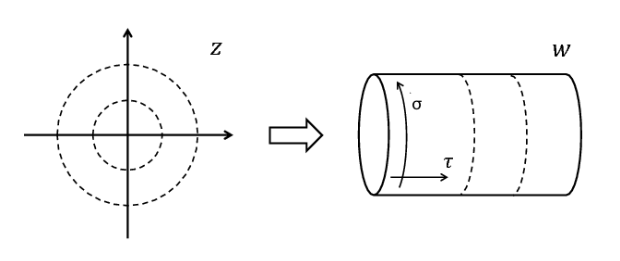
\includegraphics[width=0.9\textwidth]{img/plane_cylinder_map.png}
    \end{minipage}
    \hfill
    \begin{minipage}{0.3\textwidth}
        \caption{The conformal mapping from the complex plane to the cylinder. Concentric circles on the plane correspond to constant-time slices on the cylinder, while radial lines correspond to spatial slices.}
        \label{fig:plane_to_cylinder}
    \end{minipage}
\end{figure}

We introduce a conformal mapping from the plane coordinate \(z\) to a cylinder coordinate \(w\):
\[
    z = e^{\frac{2\pi}{L} w} \quad \text{or equivalently} \quad w = \frac{L}{2\pi} \log z.
\]
The logarithm function maps the complex plane onto an infinite strip. By imposing periodic boundary conditions, this strip rolls up seamlessly into a cylinder of circumference \(L\). If we decompose the cylinder coordinate into its real and imaginary parts, \(w = \tau + i\sigma\), and express the plane coordinate \(z\) in polar form, \(z = |z|e^{i \arg z}\), we find the relations:
\[
    \tau = \frac{L}{2\pi} \log |z| \;, \quad \sigma = \frac{L}{2\pi} \arg z.
\]
Here, \(\tau \in [-\infty, \infty]\) represents the Euclidean time evolving along the infinite length of the cylinder, while \(\sigma \in [0, L]\) is the compactified spatial coordinate wrapping around the cylinder.

This geometric mapping has profound physical implications for our quantization scheme:
\begin{itemize}
    \item Concentric circles on the \(z\)-plane (curves of constant \(|z|\)) are mapped to constant-time slices (constant \(\tau\)) on the cylinder.
    \item Radial dilatations on the plane (\(|z| \to \lambda |z|\)) correspond to time translations on the cylinder (\(\tau \to \tau + \frac{L}{2\pi} \log \lambda\)).
\end{itemize}
Consequently, the six generators of the global conformal group on the plane map directly to the six global generators on the cylinder. This transformation provides a concrete framework to quantize \(\text{CFT}_2\) using the standard QFT approach, allowing us to interpret states living on a circle and evolving radially. It also provides a powerful mechanism to control and calculate finite-size effects in critical statistical models.